\documentclass[sigconf]{acmart}
\setcopyright{none}
\settopmatter{printacmref=false, printfolios=true, authorsperrow=4}
\renewcommand\footnotetextcopyrightpermission[1]{}
\makeatletter\def\@affiliationfont{\small\normalfont}\makeatother
\usepackage{booktabs}
\begin{document}
\title{Predictive Multitask Learning for Streaming Code-Switching}
\subtitle{CS6140 Machine Learning --- Project Update 1 Report}
\author{Huanhuan Yan}\affiliation{\institution{Northeastern University}\city{Seattle}\country{USA}}\email{echoyanxx@hotmail.com}
\author{Jiaming Li}\affiliation{\institution{Northeastern University}\city{Seattle}\country{USA}}\email{ohhh668@gmail.com}
\author{Yuchen Huang}\affiliation{\institution{Northeastern University}\city{Seattle}\country{USA}}\email{huang.yuchen2@northeastern.edu}
\author{Zaixun Li}\affiliation{\institution{Northeastern University}\city{Seattle}\country{USA}}\email{zaixunli0915@gmail.com}
\renewcommand{\shortauthors}{Yan et al.}
\begin{abstract}
We study anticipatory code-switching: after reading the prefix $x_1,\dots,x_t$, predict whether the next word
$x_{t+1}$ switches language and how long the new-language span will last. This report describes the data pipeline
we built for all 15 language pairs of SwitchLingua --- language-specific word segmentation, word-level language
identification, switch and duration labels, a deduplicated 70/10/20 split, and a streaming loader whose inputs never
include $x_{t+1}$ --- and our first baselines. A naive model that only sees the current word reaches a mean
switch-class F1 of .426 across pairs (SD .102), roughly twice a model that only knows the
current word's language. Code: \url{https://github.com/StarfishJ/CS6140ML_Project}.
\end{abstract}
\maketitle
\pagestyle{plain}

\section{Problem Description}
Code-switching is the alternation between two or more languages within an utterance or conversation. Most NLP work
recognizes a switch after the mixed-language text has been observed. We instead study \textbf{anticipatory}
code-switching: at word $x_t$, using only the prefix $x_1,\dots,x_t$, predict (1) the switch label
$y_{sw}(t)=1$ if $x_{t+1}$ is in a different language than $x_t$, and (2) the duration label $y_{dur}(t)$, the length
of the new-language span starting at $x_{t+1}$: 0 for 1--2 words, 1 for 3--6, 2 for 7 or more, and $-1$ (ignored by
the loss) when there is no switch. Real-time systems such as bilingual predictive keyboards, dialogue agents and
streaming speech recognition need to know a switch is coming before it happens.
Our central question is \textbf{universality}: does one method anticipate switches equally well across typologically
different pairs? We measure it with the same pipeline and metric on every pair, reporting per-pair switch-class F1
(``Anticipatory F1'') and its standard deviation across pairs. Our final model will be a multilingual transformer
(XLM-R or mBERT) with a causal attention mask and two heads, one for $y_{sw}$ and one for $y_{dur}$.

\section{Background and Related Work}
\textbf{Code-switch prediction.} Solorio and Liu~\cite{solorio2008learning} first framed the prediction of
code-switching points in Spanish--English conversation as a learning task. They trained Naive Bayes and VFI
classifiers on lexical, part-of-speech and language-ID features of the preceding words. Results were encouraging, but
the feature-based approach was tested on one small corpus and one pair.
Ostapenko et al.~\cite{ostapenko2022speaker} predicted code-switching points in English--Spanish dialogue. They
truncated each input at a candidate point so the model sees only the prefix, and added sociolinguistic speaker
features as prompts. Speaker information improved accuracy, but evaluation covered one pair and no switch duration.
Winata et al.~\cite{winata2019synthetic} built code-switched language models for English--Mandarin. A pointer-generator
network learned where to switch between aligned parallel sentences and produced synthetic code-switched training data.
Language-model perplexity improved, but switching was modeled implicitly through the language model, on one pair.

\textbf{Language identification in code-switched text.} Solorio et al.~\cite{solorio2014overview} ran the first shared
task on word-level language identification in code-switched social-media text, for Spanish--English, Nepali--English,
Mandarin--English and Modern Standard Arabic--dialectal Arabic. Participants used CRFs and other supervised
sequence models with character and lexical features. Accuracy was high for some pairs but much lower for the closely
related Arabic varieties.
Molina et al.~\cite{molina2016overview} organized the second edition for Spanish--English and Modern Standard
Arabic--Egyptian Arabic tweets. Systems ranged from CRFs to neural networks with word and character features.
Spanish--English was again much easier than the Arabic pair, showing that closely related languages remain hard.
Aguilar et al.~\cite{aguilar2020lince} released LinCE, a benchmark of ten corpora over four pairs (including
Hindi--English and Spanish--English) and four tasks (language ID, POS tagging, NER, sentiment). They reported
baselines from BiLSTMs to multilingual BERT. Language ID is close to solved with full-sentence context, but all tasks
look at text after it is written.
Khanuja et al.~\cite{khanuja2020gluecos} proposed GLUECoS, a code-switched NLP benchmark for English--Hindi and
English--Spanish covering language ID, POS, NER, sentiment, question answering and NLI. They fine-tuned mBERT and also
pre-trained it on synthetic code-switched text. The extra pre-training helped, but the benchmark covers only two
pairs and no anticipatory task.

\textbf{Multilingual encoders.} Devlin et al.~\cite{devlin2019bert} introduced BERT, a Transformer encoder pre-trained
with masked language modeling and next-sentence prediction. Fine-tuning it set new results on eleven tasks including
GLUE and SQuAD. Its attention is bidirectional, so prefix-only prediction requires a causal mask.
Pires et al.~\cite{pires2019multilingual} probed multilingual BERT. Zero-shot transfer experiments showed that mBERT
transfers across languages and can process code-switched and transliterated input. Transfer drops for typologically
distant pairs and for transliterated text, which motivates our per-pair variance analysis.
Conneau et al.~\cite{conneau2020xlmr} trained XLM-R, a masked language model on 2.5\,TB of filtered CommonCrawl text in
100 languages. It outperformed mBERT on cross-lingual classification, QA and NER, especially for low-resource
languages. It is our strongest candidate backbone, although, like BERT, it is bidirectional.
Muller et al.~\cite{muller2021unseen} studied how multilingual models handle languages unseen in pre-training. They
found large differences between languages and that transliterating a language into the script of a related
high-resource language helps. This supports treating romanized Hindi with a model trained on romanized text.

\textbf{Multitask learning and data.} Liu et al.~\cite{liu2019mtdnn} proposed MT-DNN, which shares a BERT encoder across
tasks with task-specific output layers trained jointly. It improved GLUE results, but all tasks were sentence-level
classification over fully observed input, unlike our prefix-only switch and duration heads.
Xie et al.~\cite{xie2025switchlingua} introduced SwitchLingua, generated with the LinguaMaster multi-agent framework
under linguistic constraints, with 420K text samples across 12 languages and an audio part. It is synthetic, but it is
the only resource with the breadth of pairs a universality study needs.

\section{Dataset}
\textbf{Source.} We use the text part of SwitchLingua (SwitchLingua\_text on Hugging Face): 15 pairs,
234,172 rows, 14 X--English pairs plus German--French. Each row is a generated conversation whose
\texttt{data\_generation\_result} field is a list of utterances, with metadata such as topic and switch type. There are
no word-level language labels, so we derive them.

\textbf{Segmentation and word language ID.} Word units and language ID depend on the writing system
(Table~\ref{tab:data}). Space-separated languages are split on whitespace and punctuation, keeping combining marks
(an early version of our regex split 44.5\% of Devanagari words in the first 1,000 Hindi rows into fragments). Chinese, Cantonese and Japanese are
segmented with jieba, PyCantonese and GiNZA bunsetsu units (a content word plus its particles, comparable to the
Korean eojeol); Vietnamese syllables are merged into words by pyvi. A word mixing Latin and another script
(Korean ``presentation-eseo'') is split at the script boundary, and a hyphenated word whose parts are clearly in different
languages (``nag-meeting'') is split at the hyphen. For non-Latin pairs the Unicode script gives the language. Hindi
utterances containing Devanagari use script as well; the remaining 59.5\% of Hindi rows are
fully romanized and are tagged with \texttt{muril-hinglish-lid}, a MuRIL model fine-tuned on LinCE Hindi--English.
For the eight Latin-script pairs, a word gets the language in which it is clearly more frequent according to
wordfreq~\cite{speer2022wordfreq} (Zipf difference $\geq$1.0, or 0.5 toward English for Malay and Filipino, whose
lists contain many English loans), or the language indicated by letters only one side uses. Ambiguous words take the
language of the nearest decided words on both sides. Numbers inherit the previous word's language. On spot-checked
validation samples (about 400--500 words per Latin-script pair), word-level agreement with our own reading was about
98--99\%; these are weak labels, not gold annotations.

\textbf{Labels and split.} From the word language IDs we compute $y_{sw}$ and $y_{dur}$ for every position whose two
words have a known language (unknown words are 0.0--0.2\% of words, mostly utterance-initial numbers). Exact duplicate
rows are removed, rows that share any utterance are grouped, and groups are split 70/10/20 into train, validation and
test with a fixed seed per pair; 0 utterances appear in more than one split. Cantonese--English
(119,248 rows, 2,652 exact duplicates) is downsampled after splitting
to 8,381 rows, the median size of the other pairs.

\textbf{Streaming loader and causal inputs.} \texttt{StreamingCSDataset} is a PyTorch \texttt{IterableDataset}: a
generator reads one CSV row at a time and yields one example per word $t$ --- the window $x_{t-31},\dots,x_t$, the
language of $x_t$, $y_{sw}$ and $y_{dur}$, and optionally XLM-R/mBERT subword ids scored at the last subword of $x_t$.
Nothing is precomputed. The last word of an utterance yields no example and windows never cross utterances. Labels may
read the whole sentence, since they are the answers, but inputs never include $x_{t+1}$ in training or testing: the
text passed to a tokenizer ends at $x_t$, and the input LID is recomputed from the prefix only (left context for
Latin-script pairs, the Hinglish model run on each prefix for romanized Hindi). Re-running the pipeline on the prefix
alone for 40 validation utterances per pair gives an identical LID input in 14 pairs
(Vietnamese: 99.9\%) and an identical word $x_t$ in 12 pairs;
Cantonese, Japanese and Vietnamese match at over 99\% because their segmenters look at following characters.

\begin{table*}[t]
\caption{The 15 SwitchLingua pairs after preprocessing. Positions are word positions with a label (all splits); S/M/L
is the share of switches whose new span has 1--2 / 3--6 / 7+ words; Unk.\ is the share of words with no language.}
\label{tab:data}
\small
\begin{tabular}{lllrrrrcr}
\toprule
Pair & Segmentation & Word LID & Rows & Kept rows & Positions & Switch \% & S/M/L \% & Unk.\ \%\\
\midrule
Arabic--English & space & script & 8,548 & 8,543 & 359K & 9.1 & 41/24/35 & 0.00\\
Hindi--English & space & script+MuRIL & 8,381 & 8,380 & 444K & 26.0 & 67/22/12 & 0.02\\
Korean--English & eojeol & script & 8,266 & 8,266 & 347K & 10.6 & 40/22/38 & 0.01\\
Russian--English & space & script & 8,017 & 8,017 & 352K & 9.3 & 40/26/34 & 0.00\\
Chinese--English & jieba & script & 8,458 & 8,457 & 534K & 7.5 & 35/21/44 & 0.03\\
Cantonese--English & PyCantonese & script & 119,248 & 8,381 & 549K & 10.3 & 46/30/24 & 0.02\\
Japanese--English & GiNZA & script & 8,385 & 8,384 & 369K & 10.6 & 37/21/41 & 0.15\\
Spanish--English & space & wordfreq & 8,110 & 8,101 & 421K & 7.7 & 35/26/39 & 0.02\\
French--English & space & wordfreq & 8,070 & 8,067 & 399K & 7.1 & 34/24/42 & 0.03\\
German--English & space & wordfreq & 6,819 & 6,814 & 312K & 7.7 & 37/23/40 & 0.04\\
Italian--English & space & wordfreq & 7,979 & 7,978 & 405K & 7.1 & 34/24/43 & 0.03\\
Malay--English & space & wordfreq & 8,386 & 8,386 & 415K & 11.9 & 47/26/27 & 0.11\\
Filipino--English & space & wordfreq & 8,537 & 8,534 & 451K & 18.0 & 56/26/18 & 0.18\\
Vietnamese--English & pyvi & wordfreq & 8,457 & 8,455 & 463K & 9.3 & 43/24/33 & 0.03\\
German--French & space & wordfreq & 8,511 & 8,506 & 378K & 7.6 & 32/26/42 & 0.04\\
\midrule
Total & & & 234,172 & 123,269 & 6.20M & & & \\
\bottomrule
\end{tabular}
\end{table*}

\section{Experimentation and Results}
\textbf{Setup.} All scores are switch-class F1 on the test split (65K--110K
word positions per pair). Always stay never predicts a switch (F1 = 0 on every pair). Always switch predicts a switch
at every word; its F1 depends only on the switch rate $p$, $2p/(1+p)$, and serves as the reference line. Current LID
estimates $P(\text{switch}\mid\text{pair},\text{LID of }x_t)$ on train with add-one smoothing. The naive baseline
estimates $P(\text{switch}\mid\text{pair}, x_t)$ for the word itself, shrunk toward its language's rate with five
pseudo-counts. Both use only $x_t$ (no punctuation after it, no earlier words), and their thresholds are tuned on each
pair's validation split. Gain is naive F1 minus always-switch F1.

\begin{table}[t]
\caption{Test switch-class F1, sorted by gain of the naive (current-word) baseline over always switch.}
\label{tab:results}
\small
\begin{tabular}{lrrrr}
\toprule
Pair & Always sw. & Cur.\ LID & Naive & Gain\\
\midrule
Korean--English & .194 & .250 & \textbf{.675} & +.481\\
Japanese--English & .192 & .283 & \textbf{.524} & +.332\\
German--English & .140 & .172 & \textbf{.417} & +.278\\
German--French & .141 & .175 & \textbf{.417} & +.277\\
French--English & .132 & .163 & \textbf{.370} & +.238\\
Chinese--English & .138 & .167 & \textbf{.369} & +.231\\
Italian--English & .133 & .162 & \textbf{.347} & +.214\\
Arabic--English & .166 & .217 & \textbf{.381} & +.214\\
Hindi--English & .410 & .410 & \textbf{.624} & +.213\\
Spanish--English & .143 & .162 & \textbf{.353} & +.210\\
Filipino--English & .308 & .308 & \textbf{.491} & +.183\\
Vietnamese--English & .169 & .175 & \textbf{.349} & +.180\\
Russian--English & .171 & .200 & \textbf{.348} & +.178\\
Cantonese--English & .187 & .192 & \textbf{.364} & +.177\\
Malay--English & .212 & .212 & \textbf{.361} & +.149\\
\midrule
Mean (SD) & & .216 (.068) & \textbf{.426} (.102) & \\
\bottomrule
\end{tabular}
\end{table}

\begin{figure}[t]
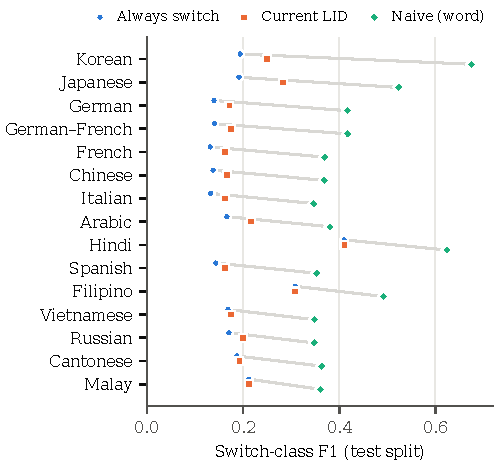
\includegraphics[width=\columnwidth]{fig_f1.pdf}
\caption{Test switch-class F1 per pair (values in Table~\ref{tab:results}). Pairs are ordered by the naive model's gain
over always switch; the grey bar joins always switch and naive.}
\label{fig:f1}
\end{figure}

\textbf{Results.} Table~\ref{tab:results} and Figure~\ref{fig:f1} show that knowing the word itself, not only its
language, roughly doubles F1: from .216 to .426 on average. The current language alone helps
little: it beats always switch by at most .091
and not at all for Hindi, Filipino and Malay, where switching is frequent and goes both ways. The naive model gains
most for Korean--English (+.481):
Korean words with the sentence-final endings \emph{-yo} / \emph{-da} are followed by a switch
97\% / 87\% of the time, against
11\% for other Korean words. It gains least for Malay--English
(+.149).
Across pairs the naive F1 has SD .102, so a single current word is far from universal; the spread is a
first measurement of the universality gap a context model must close.

\textbf{Segmentation unit.} The word unit decides how many predictions are scored. Re-running the Japanese pair with
three units (Table~\ref{tab:ja}) shows that fine morphemes add many easy no-switch positions: the switch rate falls
and current-LID F1 halves, while the naive model, which sees the word itself, loses much less. We use bunsetsu units,
comparable to Korean eojeol, so that pairs are scored on similar units.

\begin{table}[t]
\caption{Japanese--English with three segmentation units (all splits / test).}
\label{tab:ja}
\small
\begin{tabular}{lrrrr}
\toprule
Unit & Positions & Switch \% & Cur.\ LID & Naive\\
\midrule
Morphemes (fugashi) & 624K & 6.2 & .130 & .489\\
Sudachi mode C & 610K & 6.4 & .134 & .489\\
Bunsetsu (GiNZA) & 369K & 10.6 & .283 & .524\\
\bottomrule
\end{tabular}
\end{table}

\textbf{Subwords and punctuation.} With mBERT, 72\% of Korean words are split into several
subwords (English: 15\%), and with XLM-R a piece crosses into the next word for
7.6\% of Chinese and 5.1\% of Japanese words. We therefore keep labels
at the word level, score each word at its last subword, and will tokenize word by word. Inputs exclude the
punctuation after $x_t$: in SwitchLingua a sentence-final mark is followed by a switch
51--93\% of the time and precedes 4--33\%
of all switches, so models that see it score much higher on these inter-sentential switches.

\section{Plan for Next}
\begin{itemize}
\item \textbf{Causal dual-head model (Update 2).} XLM-R and mBERT with a causal attention mask, switch and duration
heads on $h_t$, loss $\lambda_1 L_{sw}+\lambda_2 L_{dur}$ with \texttt{ignore\_index}$=-1$; check against the
prefix-by-prefix loader, which must give identical predictions.
\item \textbf{Stronger baselines.} Previous plus current word, logistic regression on prefix features, a
duration-majority baseline, and a variant that sees punctuation, reported separately.
\item \textbf{Label quality.} A small hand-checked gold set per pair to measure word-LID and switch-boundary
accuracy, and incremental segmentation of the prefix for Chinese, Japanese and Vietnamese.
\item \textbf{Analysis.} Per-pair F1 bar chart and SD for each backbone, duration accuracy at true switches, and
inter- versus intra-sentential switches using SwitchLingua's switch-type field; a streaming demo at the end.
\end{itemize}

\bibliographystyle{ACM-Reference-Format}
\bibliography{references}
\end{document}
